
%{{第五十四回}}{第五十四回}}

\chapter{史太君破陈腐旧套 王熙凤效戏彩斑衣}\label{part0058_split_000.htmlux5cux23calibre_pb_0}

{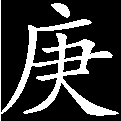
\includegraphics[width=3mm]{../Images/00004}首回楔子内云``古今小说千部共成一套''云云,犹未泄真。今借老太君一写,是劝后来胸中无机轴之诸君子不可动笔作书。}

{凤姐乃太君之要紧陪堂,今题``斑衣戏彩''是作者酬我阿凤之劳,特贬贾珍琏辈之无能耳。}

{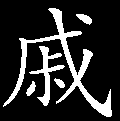
\includegraphics[width=3mm]{../Images/00005}积德于今到子孙,都中旺族首吾门。可怜立业英雄辈,遗脉谁知祖父恩。}

却说贾珍贾琏暗暗预备下大簸箩的钱,听见贾母说``赏'',他们也忙命小厮们快撒钱。只听满台钱响,贾母大悦。

二人遂起身,小厮们忙将一把新暖银壶捧在贾琏手内,随了贾珍趋至里面。贾珍先至李婶席上,躬身取下杯来,回身,贾琏忙斟了一盏;然后便至薛姨妈席上,也斟了。二人忙起身笑说:``二位爷请坐着罢了,何必多礼。''于是除邢王二夫人,满席都离了席,俱垂手旁侍。贾珍等至贾母榻前,因榻矮,二人便屈膝跪了。贾珍在先捧杯,贾琏在后捧壶。虽止二人奉酒,那贾环弟兄等,却也是排班按序,一溜随着他二人进来,见他二人跪下,也都一溜跪下。宝玉也忙跪下了。史湘云悄推他笑道:``你这会又帮着跪下作什么?有这样,你也去斟一巡酒岂不好?''宝玉悄笑道:``再等一会子再斟去。''说着,等他二人斟完起来,方起来。又与邢夫人王夫人斟过来。贾珍笑道:``妹妹们怎么样呢?''贾母等都说:``你们去罢,他们倒便宜些。''说了,贾珍等方退出。

当下天未二鼓,戏演的是《八义》中《观灯》八出。正在热闹之际,宝玉因下席往外走。贾母因说:``你往那里去!外头爆竹利害,仔细天上吊下火纸来烧了。''宝玉回说:``不往远去,只出去就来。''贾母命婆子们好生跟着。于是宝玉出来,只有麝月秋纹并几个小丫头随着。

贾母因说:``袭人怎么不见?他如今也有些拿大了,单支使小女孩子出来。''王夫人忙起身笑回道:``他妈前日没了,因有热孝,不便前头来。''贾母听了点头,又笑道:``跟主子却讲不起这孝与不孝。若是他还跟我,难道这会子也不在这里不成?皆因我们太宽了,有人使,不查这些,竟成了例了。''凤姐儿忙过来笑回道:``今儿晚上他便没孝,那园子里也须得他看着,灯烛花炮最是耽险的。这里一唱戏,园子里的人谁不偷来瞧瞧。他还细心,各处照看照看。况且这一散后宝兄弟回去睡觉,各色都是齐全的。若他再来了,众人又不经心,散了回去,铺盖也是冷的,茶水也不齐备,各色都不便宜,所以我叫他不用来,只看屋子。散了又齐备,我们这里也不耽心,又可以全他的礼,岂不三处有益。老祖宗要叫他,我叫他来就是了。''

贾母听了这话,忙说:``你这话很是,比我想的周到,快别叫他了。但只他妈几时没了,我怎么不知道。''凤姐笑道:``前儿袭人去亲自回老太太的,怎么倒忘了。''贾母想了一想笑说:``想起来了。我的记性竟平常了。''众人都笑说:``老太太那里记得这些事。''贾母因又叹道:``我想着,他从小儿伏侍了我一场,又伏侍了云儿一场,末后给了一个魔王宝玉,亏他魔了这几年。他又不是咱们家的根生土长的奴才,没受过咱们什么大恩典。他妈没了,我想着要给他几两银子发送,也就忘了。''凤姐儿道:``前儿太太赏了他四十两银子,也就是了。''

贾母听说,点头道:``这还罢了。正好鸳鸯的娘前儿也死了,我想他老子娘都在南边,我也没叫他家去走走守孝,如今叫他两个一处作伴儿去。''又命婆子将些果子、菜馔、点心之类与他两个吃去。琥珀笑说:``还等这会子呢,他早就去了。''说着,大家又吃酒看戏。

且说宝玉一径来至园中,众婆子见他回房,便不跟去,只坐在园门里茶房里烤火,和管茶的女人偷空饮酒斗牌。宝玉至院中,虽是灯光灿烂,却无人声。麝月道:``他们都睡了不成?咱们悄悄的进去唬他们一跳。''于是大家蹑足潜踪的进了镜壁一看,只见袭人和一人二人对面都歪在地炕上,那一头有两三个老嬷嬷打盹。

宝玉只当他两个睡着了,才要进去,忽听鸳鸯叹了一声,说道:``可知天下事难定。论理你单身在这里,父母在外头,每年他们东去西来,没个定准,想来你是不能送终的了,偏生今年就死在这里,你倒出去送了终。''袭人道:``正是。我也想不到能够看父母回首。太太又赏了四十两银子,这倒也算养我一场,我也不敢妄想了。''宝玉听了,忙转身悄向麝月等道:``谁知他也来了。我这一进去,他又赌气走了,不如咱们回去罢,让他两个清清静静的说一回。袭人正一个闷着,他幸而来的好。''说着,仍悄悄的出来。

宝玉便走过山石之后去站着撩衣,麝月秋纹皆站住背过脸去,口内笑说:``蹲下再解小衣,仔细风吹了肚子。''后面两个小丫头子知是小解,忙先出去茶房预备去了。这里宝玉刚转过来,只见两个媳妇子迎面来了,问是谁,秋纹道:``宝玉在这里,你大呼小叫,仔细唬着罢。''那媳妇们忙笑道:``我们不知道,大节下来惹祸了。姑娘们可连日辛苦了。''说着,已到了跟前。

麝月等问:``手里拿的是什么?''媳妇们道:``是老太太赏金、花二位姑娘吃的。''秋纹笑道:``外头唱的是《八义》,没唱《混元盒》,那里又跑出`金花娘娘'来了。''宝玉笑命:``揭起来我瞧瞧。''秋纹麝月忙上去将两个盒子揭开。两个媳妇忙蹲下身子,{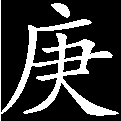
\includegraphics[width=3mm]{../Images/00004}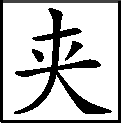
\includegraphics[width=3mm]{../Images/00012}\footnotesize \kaishu 细腻之极!一部大观园之文皆若食肥蟹,至此一句,则又三月于镇江江上啖出网之鲜鲥矣。}宝玉看了两盒内都是席上所有的上等果品菜馔,点了一点头,迈步就走。麝月二人忙胡乱掷了盒盖,跟上来。宝玉笑道:``这两个女人倒和气,会说话,他们天天乏了,倒说你们连日辛苦,倒不是那矜功自伐的。''麝月道:``这好的也很好,那不知礼的也太不知礼。''宝玉笑道:``你们是明白人,耽待他们是粗笨可怜的人就完了。''一面说,一面来至园门。

那几个婆子虽吃酒斗牌,却不住出来打探,见宝玉来了,也都跟上了。来至花厅后廊上,只见那两个小丫头一个捧着小沐盆,一个搭着手巾,又拿着沤子壶在那里久等。秋纹先忙伸手向盆内试了一试,说道:``你越大越粗心了,那里弄的这冷水。''小丫头笑道:``姑娘瞧瞧这个天,我怕水冷,巴巴的倒的是滚水,这还冷了。''

正说着,可巧见一个老婆子提着一壶滚水走来。小丫头便说:``好奶奶,过来给我倒上些。''那婆子道:``哥哥儿,这是老太太泡茶的,劝你走了舀去罢,那里就走大了脚。''秋纹道:``凭你是谁的,你不给?我管把老太太茶吊子倒了洗手。''那婆子回头见是秋纹,忙提起壶来就倒。秋纹道:``够了。你这么大年纪也没个见识,谁不知是老太太的水!要不着的人就敢要了。''婆子笑道:``我眼花了,没认出这姑娘来。''宝玉洗了手,那小丫头子拿小壶倒了些沤子在他手内,宝玉沤了。秋纹麝月也趁热水洗了一回,沤了,跟进宝玉来。

宝玉便要了一壶暖酒,也从李婶薛姨妈斟起,二人也让坐。贾母便说:``他小,让他斟去,大家倒要干过这杯。''说着,便自己干了。邢王二夫人也忙干了,让他二人。薛李也只得干了。贾母又命宝玉道:``连你姐姐妹妹一齐斟上,不许乱斟,都要叫他干了。''宝玉听说,答应着,一一按次斟了。

至黛玉前,偏他不饮,拿起杯来,放在宝玉唇上边,宝玉一气饮干。黛玉笑说:``多谢。''宝玉替他斟上一杯。凤姐儿便笑道:``宝玉,别喝冷酒,仔细手颤,明儿写不得字,拉不得弓。''宝玉忙道:``没有吃冷酒。''凤姐儿笑道:``我知道没有,不过白嘱咐你。''然后宝玉将里面斟完,只除贾蓉之妻是丫头们斟的。复出至廊上,又与贾珍等斟了。坐了一回,方进来仍归旧坐。

一时上汤后,又接献元宵来。贾母便命将戏暂歇歇:``小孩子们可怜见的,也给他们些滚汤滚菜的吃了再唱。''又命将各色果子元宵等物拿些与他们吃去。

一时歇了戏,便有婆子带了两个门下常走的女先儿进来,放两张杌子在那一边命他坐了,将弦子琵琶递过去。贾母便问李薛听何书,他二人都回说:``不拘什么都好。''贾母便问:``近来可有添些什么新书?''那两个女先儿回说道:``倒有一段新书,是残唐五代的故事。''贾母问是何名,女先儿道:``叫做《凤求鸾》。''贾母道:``这一个名字倒好,不知因什么起的,先大概说说原故,若好再说。''女先儿道:``这书上乃说残唐之时,有一位乡绅,本是金陵人氏,名唤王忠,曾做过两朝宰辅,如今告老还家,膝下只有一位公子,名唤王熙凤。''

众人听了,笑将起来。贾母笑道:``这重了我们凤丫头了。''媳妇忙上去推他,``这是二奶奶的名字,少混说。''贾母笑道:``你说,你说。''女先生忙笑着站起来,说:``我们该死了,不知是奶奶的讳。''凤姐儿笑道:``怕什么,你们只管说罢,重名重姓的多呢。''

女先生又说道:``这年王老爷打发了王公子上京赶考,那日遇见大雨,进到一个庄上避雨。谁知这庄上也有个乡绅,姓李,与王老爷是世交,便留下这公子住在书房里。这李乡绅膝下无儿,只有一位千金小姐。这小姐芳名叫作雏鸾,琴棋书画,无所不通。''贾母忙道:``怪道叫作《凤求鸾》。不用说,我猜着了,自然是这王熙凤要求这雏鸾小姐为妻。''女先儿笑道:``老祖宗原来听过这一回书。''众人都道:``老太太什么没听过!便没听过,也猜着了。''

贾母笑道:``这些书都是一个套子,左不过是些佳人才子,最没趣儿。把人家女儿说的那样坏,还说是佳人,编的连影儿也没有了。开口都是书香门第,父亲不是尚书就是宰相,生一个小姐必是爱如珍宝。这小姐必是通文知礼,无所不晓,竟是个绝代佳人。只一见了一个清俊的男人,不管是亲是友,便想起终身大事来,父母也忘了,书礼也忘了,鬼不成鬼,贼不成贼,那一点儿是佳人?便是满腹文章,做出这些事来,也算不得是佳人了。比如男人满腹文章去作贼,难道那王法就说他是才子,就不入贼情一案不成?可知那编书的是自己塞了自己的嘴。再者,既说是世宦书香大家小姐都知礼读书,连夫人都知书识礼,便是告老还家,自然这样大家人口不少,奶母丫鬟伏侍小姐的人也不少,怎么这些书上,凡有这样的事,就只小姐和紧跟的一个丫鬟?你们白想想,那些人都是管什么的,可是前言不答后语?''

众人听了,都笑说:``老太太这一说,是谎都批出来了。''贾母笑道:``这有个原故:编这样书的,有一等妒人家富贵,或有求不遂心,所以编出来污秽人家。再一等,他自己看了这些书看魔了,他也想一个佳人,所以编了出来取乐。何尝他知道那世宦读书家的道理!别说他那书上那些世宦书礼大家,如今眼下真的,拿我们这中等人家说起,也没有这样的事,别说是那些大家子。可知是诌掉了下巴的话。所以我们从不许说这些书,丫头们也不懂这些话。这几年我老了,他们姊妹们住的远,我偶然闷了,说几句听听,他们一来,就忙歇了。''李薛二人都笑说:``这正是大家的规矩,连我们家也没这些杂话给孩子们听见。''

凤姐儿走上来斟酒,笑道:``罢,罢,酒冷了,老祖宗喝一口润润嗓子再掰谎。这一回就叫作《掰谎记》,就出在本朝本地本年本月本日本时,老祖宗一张口难说两家话,花开两朵,各表一枝,是真是谎且不表,再整那观灯看戏的人。老祖宗且让这二位亲戚吃一杯酒看两出戏之后,再从昨朝话言掰起如何?''他一面斟酒,一面笑说,未曾说完,众人俱已笑倒。两个女先儿也笑个不住,都说:``奶奶好刚口。奶奶要一说书,真连我们吃饭的地方也没了。''薛姨妈笑道:``你少兴头些,外头有人,比不得往常。''凤姐儿笑道:``外头的只有一位珍大爷。我们还是论哥哥妹妹,从小儿一处淘气了这么大。这几年因做了亲,我如今立了多少规矩了。便不是从小儿的兄妹,便以伯叔论,那《二十四孝》上`斑衣戏彩',他们不能来`戏彩'引老祖宗笑一笑,我这里好容易引的老祖宗笑了一笑,多吃了一点儿东西,大家喜欢,都该谢我才是,难道反笑话我不成?''贾母笑道:``可是这两日我竟没有痛痛的笑一场,倒是亏他,才一路笑的我心里痛快了些,我再吃一钟酒。''吃着酒,又命宝玉:``也敬你姐姐一杯。''凤姐儿笑道:``不用他敬,我讨老祖宗的寿罢。''说着,便将贾母的杯拿起来,将半杯剩酒吃了,将杯递与丫鬟,另将温水浸的杯换了一个上来。于是各席上的杯都撤去,另将温水浸着待换的杯斟了新酒上来,然后归坐。

女先儿回说:``老祖宗不听这书,或者弹一套曲子听听罢。''贾母便说道:``你们两个对一套《将军令》罢。''二人听说,忙和弦按调拨弄起来。贾母因问:``天有几更了。''众婆子忙回:``三更了。''贾母道:``怪道寒浸浸的起来。''早有众丫鬟拿了添换的衣裳送来。王夫人起身笑说道:``老太太不如挪进暖阁里地炕上倒也罢了。这二位亲戚也不是外人,我们陪着就是了。''贾母听说,笑道:``既这样说,不如大家都挪进去,岂不暖和?''王夫人道:``恐里间坐不下。''贾母笑道:``我有道理。如今也不用这些桌子,只用两三张并起来,大家坐在一处挤着,又亲香,又暖和。''众人都道:``这才有趣。''说着,便起了席。众媳妇忙撤去残席,里面直顺并了三张大桌,另又添换了果馔摆好。贾母便说:``这都不要拘礼,只听我分派你们就坐才好。''说着便让薛李正面上坐,自己西向坐了,叫宝琴、黛玉、湘云三人皆紧依左右坐下,向宝玉说:``你挨着你太太。''于是邢夫人王夫人之中夹着宝玉,宝钗等姊妹在西边,挨次下去便是娄氏带着贾菌,尤氏李纨夹着贾兰,下面横头便是贾蓉之妻。贾母便说:``珍哥儿带着你兄弟们去罢,我也就睡了。''

贾珍等忙答应,又都进来。贾母道:``快去罢!不用进来,才坐好了,又都起来。你快歇着,明日还有大事呢。''贾珍忙答应了,又笑说:``留下蓉儿斟酒才是。''贾母笑道:``正是忘了他。''贾珍答应了一个``是'',便转身带领贾琏等出来。二人自是欢喜,便命人将贾琮贾璜各自送回家去,便邀了贾琏去追欢买笑,不在话下。

这里贾母笑道:``我正想着虽然这些人取乐,竟没一对双全的,就忘了蓉儿。这可全了,蓉儿就合你媳妇坐在一处,倒也团圆了。''因有媳妇回说开戏,贾母笑道:``我们娘儿们正说的兴头,又要吵起来。况且那孩子们熬夜怪冷的,也罢,叫他们且歇歇,把咱们的女孩子们叫了来,就在这台上唱两出给他们瞧瞧。''媳妇听了,答应了出来,忙的一面着人往大观园去传人,一面二门口去传小厮们伺候。小厮们忙至戏房将班中所有的大人一概带出,只留下小孩子们。

一时,梨香院的教习带了文官等十二个人,从游廊角门出来。婆子们抱着几个软包,因不及抬箱,估料着贾母爱听的三五出戏的彩衣包了来。婆子们带了文官等进去见过,只垂手站着。贾母笑道:``大正月里,你师父也不放你们出来逛逛。你等唱什么?刚才八出《八义》闹得我头疼,咱们清淡些好。你瞧瞧,薛姨太太这李亲家太太都是有戏的人家,不知听过多少好戏的。这些姑娘们都比咱们家姑娘见过好戏,听过好曲子。如今这小戏子又是那有名玩戏家的班子,虽是小孩子们,却比大班还强。咱们好歹别落了褒贬,少不得弄个新样儿的。叫芳官唱一出《寻梦》,只提琴至管箫合,笙笛一概不用。\href{../Text/part0058_split_000.html\#lnkback_1_a}{\textsuperscript{①}}''文官笑道:``这也是的,我们的戏自然不能入姨太太和亲家太太姑娘们的眼,不过听我们一个发脱口齿,再听一个喉咙罢了。''贾母笑道:``正是这话了。''李婶薛姨妈喜的都笑道:``好个灵透孩子,他也跟着老太太打趣我们。''贾母笑道:``我们这原是随便的顽意儿,又不出去做买卖,所以竟不大合时。''说着又道:``叫葵官唱一出《惠明下书》,也不用抹脸。只用这两出叫他们听个疏异罢了。若省一点力,我可不依。''

文官等听了出来,忙去扮演上台,先是《寻梦》,次是《下书》。众人都鸦雀无闻,薛姨妈因笑道:``实在亏他,戏也看过几百班,从没见用箫管的。''贾母道:``也有,只是像方才《西楼·楚江晴》一支,多有小生吹箫和的。这大套的实在少,这也在主人讲究不讲究罢了。这算什么出奇?''指湘云道:``我像他这么大的时节,他爷爷有一班小戏,偏有一个弹琴的凑了来,即如《西厢记》的《听琴》,《玉簪记》的《琴挑》,《续琵琶》的《胡笳十八拍》,竟成了真的了,比这个更如何?''众人都道:``这更难得了。''贾母便命个媳妇来,吩咐文官等叫他们吹一套《灯月圆》。媳妇领命而去。

当下贾蓉夫妻二人捧酒一巡,凤姐儿因见贾母十分高兴,便笑道:``趁着女先儿们在这里,不如叫他们击鼓,咱们传梅,行一个`春喜上眉梢'的令如何?''贾母笑道:``这是个好令,正对时对景。''忙命人取了一面黑漆铜钉花腔令鼓来,与女先儿们击着,席上取了一枝红梅。贾母笑道:``若到谁手里住了,吃一杯,也要说个什么才好。''凤姐儿笑道:``依我说,谁像老祖宗要什么有什么呢。我们这不会的,岂不没意思。依我说也要雅俗共赏,不如谁输了谁说个笑话罢。''众人听了,都知道他素日善说笑话,最是他肚内有无限的新鲜趣谈。今儿如此说,不但在席的诸人喜欢,连地下伏侍的老小人等无不欢喜。那小丫头子们都忙出去,找姐唤妹的告诉他们:``快来听,二奶奶又说笑话儿了。''众丫头子们便挤了一屋子。于是戏完乐罢。贾母命将些汤点果菜与文官等吃去,便命响鼓。那女先儿们皆是惯的,或紧或慢,或如残漏之滴,或如迸豆之疾,或如惊马之乱驰,或如疾电之光而忽暗。其鼓声慢,传梅亦慢;鼓声疾,传梅亦疾。恰恰至贾母手中,鼓声忽住。大家呵呵一笑,贾蓉忙上来斟了一杯。众人都笑道:``自然老太太先喜了,我们才托赖些喜。''贾母笑道:``这酒也罢了,只是这笑话倒有些个难说。''众人都说:``老太太的比凤姐儿的还好还多,赏一个我们也笑一笑儿。''

贾母笑道:``并没什么新鲜发笑的,少不得老脸皮子厚的说一个罢了。''因说道:``一家子养了十个儿子,娶了十房媳妇。惟有第十个媳妇最聪明伶俐,心巧嘴乖,公婆最疼,成日家说那九个不孝顺。这九个媳妇委屈,便商议说:`咱们九个心里孝顺,只是不像那小蹄子嘴巧,所以公公婆婆老了,只说他好,这委屈向谁诉去?'大媳妇有主意,便说道:`咱们明儿到阎王庙去烧香,和阎王爷说去,问他一问,叫我们托生人,为什么单单的给那小蹄子一张乖嘴,我们都是笨的。'众人听了都喜欢,说这主意不错。第二日便都到阎王庙里来烧了香,九个人都在供桌底下睡着了。九个魂专等阎王驾到,左等不来,右等也不到。正着急,只见孙行者驾着筋斗云来了,看见九个魂便要拿金箍棒打,唬得九个魂忙跪下央求。孙行者问原故,九个人忙细细的告诉了他。孙行者听了,把脚一跺,叹了一口气道:`这原故幸亏遇见我,等着阎王来了,他也不得知道的。'九个人听了,就求说:`大圣发个慈悲,我们就好了。'孙行者笑道:`这却不难。那日你们妯娌十个托生时,可巧我到阎王那里去的,因为撒了泡尿在地下,你那小婶子便吃了。你们如今要伶俐嘴乖,有的是尿,再撒泡你们吃了就是了。'''说毕,大家都笑起来。

凤姐儿笑道:``好的,幸而我们都笨嘴笨腮的,不然也就吃了猴儿尿了。''尤氏娄氏都笑向李纨道:``咱们这里谁是吃过猴儿尿的,别装没事人儿。''薛姨妈笑道:``笑话儿不在好歹,只要对景就发笑。''说着又击起鼓来。小丫头子们只要听凤姐儿的笑话,便俏俏的和女先儿说明,以咳嗽为记。须臾传至两遍,刚到了凤姐儿手里,小丫头子们故意咳嗽,女先儿便住了。

众人齐笑道:``这可拿住他了。快吃了酒说一个好的,别太逗的人笑的肠子疼。''凤姐儿想了一想,笑道:``一家子也是过正月半,合家赏灯吃酒,真真的热闹非常,祖婆婆、太婆婆、婆婆、媳妇、孙子媳妇、重孙子媳妇、亲孙子、侄孙子、重孙子、灰孙子、滴滴搭搭的孙子、孙女儿、外孙女儿、姨表孙女儿、姑表孙女儿,\ldots{}\ldots{}嗳哟哟,真好热闹!''众人听他说着,已经笑了,都说:``听数贫嘴,又不知编派那一个呢?''尤氏笑道:``你要招我,我可撕你的嘴。''凤姐儿起身拍手笑道:``人家费力说,你们混,我就不说了。''贾母笑道:``你说你说,底下怎么样?''凤姐儿想了一想,笑道:``底下就团团的坐了一屋子,吃了一夜酒就散了。''众人见他正言厉色的说了,别无他话,都怔怔的还等下话,只觉冰冷无味。

史湘云看了他半日,凤姐儿笑道:``再说一个过正月半的。几个人抬着个房子大的炮仗往城外放去,引了上万的人跟着瞧去。有一个性急的人等不得,便偷着拿香点着了。只听`噗哧'一声,众人哄然一笑都散了。这抬炮仗的人抱怨卖炮仗的扞的不结实,没等放就散了。''湘云道:``难道他本人没听见响?''凤姐儿道:``这本人原是聋子。''众人听说,一回想,不觉一齐失声都大笑起来。又想着先前那一个没完的,问他:``先一个怎么样?也该说完。''凤姐儿将桌子一拍,说道:``好罗唆,到了第二日是十六日,年也完了,节也完了,我看着人忙着收东西还闹不清,那里还知道底下的事了。''众人听说,复又笑将起来。凤姐儿笑道:``外头已经四更,依我说,老祖宗也乏了,咱们也该`聋子放炮仗------散了'罢。''尤氏等用手帕子握着嘴,笑的前仰后合,指他说道:``这个东西真会数贫嘴。''贾母笑道:``真真这凤丫头越发贫嘴了。''一面说,一面吩咐道:``他提炮仗来,咱们也把烟火放了解解酒。''

贾蓉听了,忙出去带着小厮们就在院内安下屏架,将烟火设吊齐备。这烟火皆系各处进贡之物,虽不甚大,却极精巧,各色故事俱全,夹着各色花炮。林黛玉禀气柔弱,不禁毕驳之声,贾母便搂他在怀中。薛姨妈搂着湘云。湘云笑道:``我不怕。''宝钗等笑道:``他专爱自己放大炮仗,还怕这个呢。''王夫人便将宝玉搂入怀内。凤姐儿笑道:``我们是没有人疼的了。''尤氏笑道:``有我呢,我搂着你。也不怕臊,你这孩子又撒娇了,听见放炮仗,吃了蜜蜂儿屎的,今儿又轻狂起来。''凤姐儿笑道:``等散了,咱们园子里放去。我比小厮们还放的好呢。''

说话之间,外面一色一色的放了又放,又有许多的满天星、九龙入云、一声雷、飞天十响之类的零碎小爆竹。放罢,然后又命小戏子打了一回``莲花落'',撒了满台钱,命那孩子们满台抢钱取乐。又上汤时,贾母说道:``夜长,觉的有些饿了。''凤姐儿忙回说:``有预备的鸭子肉粥。''贾母道:``我吃些清淡的罢。''凤姐儿忙道:``也有枣儿熬的粳米粥,预备太太们吃斋的。''贾母笑道:``不是油腻腻的就是甜的。''凤姐儿又忙道:``还有杏仁茶,只怕也甜。''贾母道:``倒是这个还罢了。''说着,又命人撤去残席,外面另设上各种精致小菜。大家随便随意吃了些,用过漱口茶,方散。

十七日一早,又过宁府行礼,伺候掩了宗祠,收过影像,方回来。此日便是薛姨妈家请吃年酒。十八日便是赖大家,十九日便是宁府赖升家,二十日便是林之孝家,二十一日便是单大良家,二十二日便是吴新登家。这几家,贾母也有去的,也有不去的,也有高兴直待众人散了方回的,也有兴尽半日一时就来的。凡诸亲友来请或来赴席的,贾母一概怕拘束不会,自有邢夫人、王夫人、凤姐儿三人料理。连宝玉只除王子腾家去了,馀者亦皆不会,只说贾母留下解闷。所以倒是家下人家来请,贾母可以自便之处,方高兴去逛逛。闲言不提,且说当下元宵已过------

{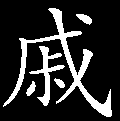
\includegraphics[width=3mm]{../Images/00005}总评:读此回者凡三变。不善读者徒赞其如何演戏、如何行令、如何挂花灯、如何放爆竹,目眩耳聋,应接不暇。少解读者,赞其座次有伦、巡酒有度,从演戏渡至女先,从女先渡至凤姐,从凤姐渡至行令,从行令渡至放花爆:脱卸下来,井然秩然,一丝不乱。会读者须另具卓识,单着眼史太君一席话,将普天下不近理之``奇文''、不近情之``妙作''一齐抹倒。是作者借他人酒杯,消自己{{(傀儡)}}{[}块垒{]},画一幅行乐图,铸一面菱花镜,为全部总评。噫!作者已逝,圣叹云亡,愚不自量,辄拟数语,知我罪我,其听之矣。}

{\href{../Text/part0058_split_000.html\#navto_1_a}{①}此句疑有错夺。有人断为``只提琴,至管箫合笙笛一概不用。''语气更顺畅,但与后文薛姨妈说的``从没见用箫管的''矛盾。暂保留目前的标点。}
